\documentclass[11pt,a4paper,pointlessnumbers]{scrreprt}  % [Schriftgröße, Abmaße Seite, keine Punkte hinter letzter gliederungsnummer und bildnummerierungen] {dokumentenklasse}

\usepackage[utf8]{inputenc}			% für Umlaute
\usepackage[T1]{fontenc}			% für Sonderzeichen
\usepackage{lmodern}				% latinmodern
\usepackage[german] {babel}% languages
\usepackage{mathtools}
\usepackage{empheq}
\usepackage{subfigure}

%\usepackage{mathptmx}				% Schriftart Arial
%\usepackage[scaled]{helvet}			% Schriftart Arial
%\renewcommand\familydefault{phv} 	% serifenlose Schrift der Schriftart einfügen (nicht zu empfehlen bei langen Texten)

\usepackage{amssymb,amsmath,amstext}% mathamatical calculation

\usepackage{graphicx} 		% for including graphics

\usepackage{geometry}				% für seitenränder	
\geometry{
	left=3cm,
	right=2.5cm,
	top=3cm,
	bottom=2.5cm
	}
	
\usepackage{setspace}				% für Zeilenabstände, Absatzabstände
\onehalfspacing						% 1,5-facher Zeilenabstand		

\setlength{\parindent}{0em} 		% verhindert das einrücken der ersten Zeile eines jeden Absatzes
\setlength{\parskip}{6pt}			% Abstand zwischen Absätzen

\usepackage[automark]{scrpage2}		% settings header and footer
\pagestyle{scrheadings}
\clearscrheadfoot

\ihead{\headmark}					% settings header
\setheadsepline{0.5pt}
%\topmargin-10mm
%\headsep10mm

%\ifoot{Markus Noack}				% settings footer
%\cfoot{Beschreibung von Wachstums- und Verdrängungsprozessen in der Systembiologie mit Zellulären Automaten}						
\ofoot{\pagemark}
\setfootsepline{0.5pt}
\footskip12.5mm

\renewcommand*\chapterpagestyle{scrheadings}

\newcommand{\CS}{C\nolinebreak\hspace{-.05em}\raisebox{.6ex}{\scriptsize\bf \#}}

\usepackage{chngcntr}
%\counterwithout{equation}{chapter}

\usepackage{url}

\usepackage{textcomp}				% text symbols  copyright, trademark, Celsius,...
\usepackage[labelfont=bf]{caption}	% bold name and number of the captions of pictures and tables

\usepackage{tabularx}
\usepackage{booktabs}
\renewcommand{\arraystretch}{1.2}


\begin{document}
	\begin{titlepage}
		\centering
		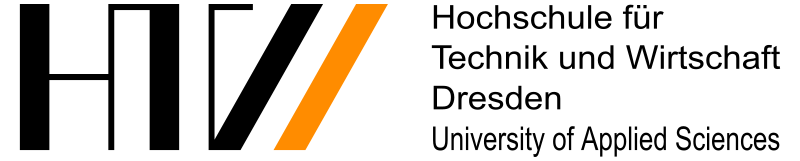
\includegraphics[width=0.5\textwidth]{Htw-dresden-logo}\par\vspace{1cm}
		{\scshape\Large Forschungs- und Entwicklungsprojekt 17/18\par}
		\vspace{1.5cm}
		{\huge\bfseries Beschreibung von Wachstums- und
			Verdrängungsprozessen in der Systembiologie mit
			Zellulären Automaten\par}
		\vspace{2cm}
		{\Large\itshape Markus Noack\par}
		\vfill
		Betreut von\par
		Prof. Dr. Anja Voß-Böhme
		
		\vfill
		
		% Bottom of the page
		{\large \today\par}
	\end{titlepage}

\tableofcontents 

\chapter{Zielstellung}
\pagenumbering {arabic}
Zellen bilden die kleinste Einheit allen Lebens. Seit ihrer Entdeckung vor über 350 Jahren wird ihr Verhalten eingehend studiert und obwohl mittlerweile ein gutes Verständnis für die Prozesse auf zellulärer Ebene besteht, ist die Regulierung und Steuerung dieser Prozesse noch nicht vollständig ergründet. \par
Im Rahmen des Forschungs- und Entwicklungsprojekts 2017/2018 des Masterstudiengangs Angewandte Informationstechnologien soll die Frage beantwortet werden, ob sich Zellverhalten mittels eines zellulären Automaten (nachfolgend CA abgekürzt) beschreiben und vor allem erklären lässt. \par
Ziel des Projektes ist es, aufbauend auf den Ergebnissen eines Vorprojektes einen CA zu entwickeln, der die Wachstums- und Verdrängungsprozesse in der Systembiologie möglichst realistisch abbildet und somit zum Verständnis dieser beitragen kann.\par 
Mit Hilfe eines funktionsfähigen Automaten könnte man noch unbekannte Korrelationen erkennen, die unter Umständen mit derzeitigen technischen Mitteln nicht messbar sind. Des Weiteren könnte man ihn nutzen um Vorhersagen zu treffen, zum Beispiel wie eine Verletzung heilen wird oder wie ein Tumor sich ausbreitet.\par

Diese Arbeit schätzt den abschließenden Forschungsprojektstand nach den zwei für die Bearbeitung vorgesehenen Semester ein. Um einen verständlichen Einstieg in das Thema zu geben, werden zunächst CA im Allgemeinen und damit einhergehende Begrifflichkeiten beschrieben. Anschließend wird ein Überblick über die bereits im Vorfeld dieser Arbeit bestehende Vorarbeit gegeben. Im Kapitel Methodik wird die Herangehensweise an das Projekt beschrieben. Darauf folgt ein Kapitel über die konzeptionellen Vorgaben an den CA. Im nächsten Kapitel wird aus den Vorgaben zunächst ein mathematisches Modell abgeleitet, bevor im nächsten Kapitel dessen programmatische Umsetzung beschrieben wird. Abschließend werden die bei der bisherigen Implementierung gewonnenen Ergebnisse evaluiert und ein Ausblick für eine mögliche Weiterarbeit gegeben.
 
\chapter{Zelluläre Automaten}
In diesem Kapitel wird das Konzept zellulärer Automaten und aller damit einhergehender Begrifflichkeiten beschrieben.
Dabei wird bewusst auf eine mathematische Beschreibung zellulärer Automaten verzichtet, da diese ausführlich im Kapitel mathematisches Modell erfolgt. \par
CA ordnen sich in die Kategorie der diskreten Simulationen ein. Grundlage stellt dabei ein diskreter Raum dar, der auch oft als Spielfeld oder Gitter bezeichnet wird. Dieser Raum kann beliebige Dimensionen haben, wobei ein zweidimensionaler Raum wie in Abbildung \ref{fig:Zustand} gängig ist. 

\begin{figure}[!ht]
	\centering
	\includegraphics{Zustandsfaerbung}
	\caption{Zweidimensionaler CA mit 7x6 Gitterzellen \cite{Scholz2014}}
	\label{fig:Zustand}
\end{figure}

Die einzelnen Gitterzellen des Automaten können durch festgelegte Regeln ihren Zustand wechseln. Die Zustandswechsel erfolgen in diskreten Zeitschritten. Das Besondere an zellulären Automaten ist, dass die Interaktion der Gitterzellen meist auf Nachbarschaften beschränkt sind, wobei diese für jede Zelle gleich definiert sind. Darum eignen sie sich gut um die Interaktionen auf biologischer Zellebene darzustellen, da Wachstum und Bewegung dort ebenfalls räumlich lokal beeinflusst werden. Es gibt mehrere Möglichkeiten zur Definition der Nachbarschaften. Abbildung \ref{fig:Neumann} und Abbildung \ref{fig:Moore} stellen die bekanntesten Nachbarschaftsbeziehungen dar.\newpage

\begin{figure}[!ht]
	\vspace{2cm}
	\subfigure[Von-Neumann-Nachbarschaft ]{\includegraphics[width=0.5\textwidth]{NeumannNachbarschaft}\label{fig:Neumann}} 
	\subfigure[Moore-Nachbarschaft ]{\includegraphics[width=0.5\textwidth]{MooreNachbarschaft}\label{fig:Moore}} 
	\caption{Nachbarschaftsbeziehungen \cite{Scholz2014}} 
	\label{fig:Nachbarschaftsbeziehungen}
\end{figure} 

Für den Fall, dass eine Gitterzelle am Rand des Spielfelds liegt und somit keine komplette Nachbarschaft innerhalb des Felds besitzt, müssen Randbedingungen definiert werden. Man unterscheidet zwischen abgeschlossenen und periodischen Randbedingungen. Bei einem abgeschlossenen Rand wird davon ausgegangen, dass Randzellen eingeschränkte Nachbarschaften haben und somit weniger Optionen für einen Zustandswechsel. Periodische Ränder hingegen ergänzen die fehlende Nachbarschaft durch Zellen vom gegenüberliegenden Rand. \par

Da wie bereits zu Beginn erwähnt, an die Vorarbeit von zwei Studenten angeknüpft wurde, werden im nächsten Abschnitt deren bisherige Ergebnisse vorgestellt, bevor der derzeitige Projektfortschritt beleuchtet wird.


\chapter{Vorarbeit}
Hauptziel des bisherigen Projektverlaufs war es, den biologischen Sachverhalt durch unterschiedliche Modelle zu realisieren und diverse Darstellungsmöglichkeiten zu vergleichen. Damit einhergehend wurde eine Webanwendung entwickelt, die in zwei Darstellungsformen (Graphen-basiert: Abbildung \ref{fig:Graphenbasiert} \& Klassisch: Abbildung \ref{fig:Klassisch}) unterteilt ist. 

\begin{figure}[!ht]
	\centering
	\subfigure[Graphen-basierte Darstellung ]{\includegraphics[width=7cm,height=7cm]{Graphenbasiert}\label{fig:Graphenbasiert}} 
	\subfigure[Klassischer CA ]{\includegraphics[width=7cm,height=7cm]{KlassischerCA}\label{fig:Klassisch}} 
	\caption{Darstellungsformen der Webanwendung \cite{Zellsimulator}} 
\end{figure} 

Zudem wurden die Ergebnisse der beiden Simulationen mit den Ergebnissen der Simulationssoftware Morpheus verglichen. Morpheus basiert auf dem Cellular Potts Model und verfolgt einen deutlich komplexeren Simulationsansatz als zelluläre Automaten. Umso erstaunlicher ist es, dass mit allen drei Simulationen vergleichbare Resultate erzielt werden konnten. Der klassische CA-Ansatz hat sich dabei als am vielversprechendsten herausgestellt und sollte im weiteren Verlauf verfolgt werden. Da eine mit der Systembiologie vergleichbare Datengenerierung noch nicht im Vordergrund stand, wurden die Eingangsparameter des CA zum damaligen Zeitpunkt frei gewählt. Zudem beschränkte sich die Komplexität der einzelnen Simulationsschritte auf nur wenige einfache Regeln.\par
 
Die aktuelle Arbeit knüpft hier an, indem der CA an geeignete Kenngrößen der Systembiologie angepasst wird. Auf welcher Grundlage und mit welchen Mitteln dies erfolgt, wird im nächsten Kapitel beschrieben.

\chapter{Methodik}

Während der Einarbeitungsphase erregte ein Artikel von Alberto Puliafito et al. (2010) \cite{Puliafito} besondere Aufmerksamkeit. Dieser beschäftigt sich mit der Zellkontakthemmung, einer Eigenschaft von Zellen, das Zellwachstum und die Zellteilung ab einer bestimmten Zelldichte einzustellen. Der Artikel liefert dabei detaillierte Einblicke in das Wachstum von Nierenzellen. Da es sich bei den beobachteten Zellen um einlagige Gewebezellen handelt, eignen sie sich hervorragend für einen Vergleich mit einem zweidimensionalen zellulären Automaten. Eine genaue Auflistung, der dort entnommenen Kenngrößen, befindet sich in den Abschnitten über Eingabe- und Vergleichsparameter. \par 

Mit dem Hinzukommen der zahlreichen Kenngrößen und der damit steigenden Komplexität, wurde der Grundaufbau des CA überdacht. Im Zuge dessen wurde beschlossen, die bisherige Implementierung in eine \CS  -Anwendung zu migrieren. \par

Die Webanwendung hat zwar eine sehr gute Visualisierung geboten, allerdings eignet sich JavaScript aufgrund von z.B. fehlenden Parallelisierungsmöglichkeiten nicht für umfangreichere Simulationen. \par

\CS \ hingegen bietet durch die Nutzung von Threads eine deutlich performantere Grundlage für den zellulären Automaten. Zudem bietet sich mit Visual Studio eine mächtige Entwicklungsumgebung, die einfacheres Debuggen und Testen ermöglicht. Die konkrete Implementierung wird im Abschnitt Programmaufbau detaillierter beschrieben. \par 

Die von der Anwendung generierten Daten werden zum Teil direkt im Programm analysiert, sowie in eine CSV-Datei gespeichert um dann weiterverarbeitet zu werden. Die Weiterverarbeitung erfolgt in MATLAB bzw. der alternativen Open Source Lösung Octave. Gleichzeitig kann an dieser Stelle eine Visualisierung der Daten durchgeführt werden. Details dazu finden sich im Abschnitt Datengenerierung und Auswertung. 

\chapter{Konzeptionelle Vorgaben der Simulation}
Das Zellverhalten soll zunächst auf ein Zusammenspiel aus den drei Zellaktionen Bewegung, Wachstum und Teilung heruntergebrochen werden. Auf CA-Ebene spiegeln diese Aktionen Zustandsübergänge wieder. Da nicht bekannt ist welche Aktion eine Zelle in welchem Zeitschritt durchführt, wird jeder Aktion eine Wahrscheinlichkeit zugeordnet. Da ein Simulationsschritt somit eine Vielzahl von Zufallsexperimenten ist, kann man die Simulation auch als Monte-Carlo-Simulation betrachten. Ein Zeitschritt in der Simulation ist somit ein Monte-Carlo-Schritt (MCS). \par 

Die Simulation besteht aus \textit{n} hintereinander ausgeführten MCS, wobei \textit{n} so gewählt wird, dass ein Simulationsdurchlauf einen Zeitraum von 15-20 Tagen simuliert. Damit die einzelnen Wahrscheinlichkeiten der Zellaktionen sich nicht gegenseitig ausschließen, also gewährleistet wird, dass eine Zelle pro MCS die Möglichkeit hatte sich zu bewegen, zu teilen oder zu wachsen, wird jeder MCS in \textit{x} Einzelschritte unterteilt, wobei \textit{x} die Anzahl der Zellen zu Beginn des MCS mal die möglichen Zellaktionen ist. In jedem dieser Schritte werden gleichverteilt eine Zelle und eine Zellaktion ausgewählt. Anschließend wird die Aktion zu einer bestimmten Wahrscheinlichkeit ausgeführt. \par 

Somit ist gewährleistet, dass im Mittel jede Zelle die Möglichkeit hatte jede ihr möglichen Aktionen auszuführen. \par 

Da eine 1:1 Abbildung der Realität durch die Simulation aufgrund von fehlenden Informationen bzw. fehlender Rechenkapazität nicht möglich ist, müssen einige vereinfachende Annahmen für die Simulation getroffen werden. Diese werden im Folgenden ohne ausschweifende Begründung aufgelistet:

\begin{itemize}
	\item Alle Zellen eines Zelltyps sind grundsätzlich gleich, was ihr Verhalten betrifft. Lediglich externe Bedingungen beeinflussen dieses.
	\item Zellen besitzen eine minimale bzw. maximale Größe.
	\item Zellen sind flach.
	\item Zellen können nicht schrumpfen.
	\item Zellen können nicht sterben.
	\item Temperatur, Substrat, Nährstoffgehalt und sonstige Einflüsse werden als homogen und neutral angenommen und beeinflussen die Simulation somit nicht.
\end{itemize}

Für die Nachbarschaftsbeziehungen wird die im Kapitel Zelluläre Automaten beschriebene Moore-Nachbarschaft verwendet, da Zellen keine statische Form besitzen und somit in Kontakt mit mehr als 4 Nachbarn treten können. Die konkrete Zellform spielt für die Simulation keine Rolle. Das beobachtete Zellgewebe tendiert zu einer gleichmäßigen Aufteilung. Zudem fehlen momentan Informationen wie die Zellform das Zellverhalten beeinflusst.\par 

Für die Randbedingungen wird ein abgeschlossener Rand verwendet. Da der Rand die Simulation aber nicht beeinflussen soll, wird das Gitter so groß gewählt, dass Zellen den Rand in der vorgegebenen Simulationszeit nicht erreichen können. \par 

Um eine realistischere Simulation zu ermöglichen, wird von einem klassischen CA-Zustandsraum abgewichen. Klassischer Weise müsste jedem Gitterplatz(fortlaufend Knoten) eine Zelle zugeordnet werden, damit sich jeder Knoten in einem eindeutig definierten Zustand befindet. Stattdessen soll jedem Knoten eine Liste von Zellen zugeordnet werden. Der Zustandsraum wird durch ein 2D-Array aus Knoten abgebildet. Damit nicht unendlich große und viele Zellen an einem Knoten sein können, wird der Platz im Knoten durch eine Kapazität beschränkt, welche für alle Knoten gleich ist. Der Ansatz den Raum aus Knoten, anstatt direkt aus Zellen bestehen zu lassen, wurde aus mehreren Gründen gewählt. Zum einen lassen sich viele kleine Zellen auf engem Raum darstellen. Ferner lässt sich die Zelldichte an einem Ort gut bestimmen, indem man Kapazität und Zellanzahl ins Verhältnis setzt. Des Weiteren lässt sich die Zellteilung realistischer darstellen, da sich Zellen an der Stelle teilen können und keinen neuen Knoten beanspruchen. \par

Im nächsten Kapitel wird das mathematische Modell beschrieben, das sich aus den in diesem Kapitel beschriebenen Anforderungen ergibt.

\chapter{Mathematisches Modell}
\section{Beschreibung des Zustandsraumes}
Der zelluläre Automat wird durch folgende Größen definiert: 
\begin{itemize}
	%\setlength\itemsep{2em}
	\item Ein diskretes Gitter $S \subset \mathbb{Z}\textsuperscript{2}$, bestehend aus $n\textsubscript{x} \cdot n\textsubscript{y}$ Knoten, wobei $S$ ein Rechteck bildet mit Seitenlängen $n\textsubscript{x}, n\textsubscript{y} \in \mathbb{N}$. Ein Knoten wird mit $\boldsymbol{r} \in S$ bezeichnet.
	
	\item Die Nachbarschaften $N\textsubscript{$\boldsymbol{r}$}$, wobei jeder Knoten $\boldsymbol{r} = (x,y)$ 8 Nachbarn besitzt (Moore-Nachbarschaft). \par Beispiel für die Nachbarschaftsdefinition, für den im Koordinatenursprung liegenden Knoten $\vec{0} = (0,0)$: 
	\[
	N\textsubscript{$\vec{0}$} = \{(-1,0), (1,0), (-1,-1), (0,-1), (1,-1), (1,0), (1,1), (0,1)\}
	\]
	Allgemein gilt: $N\textsubscript{$\boldsymbol{r}$} = \boldsymbol{r} + N\textsubscript{$\vec{0}$}$, wobei $\boldsymbol{r} + B := \{ r+y: y\in B \}$
	%Minkowski Addition
	
	\item Knoten mit $\boldsymbol{r} = (x,y), |x|=n_{x}/2 \text{ oder } |y|=n_{y}/2$, werden als Randknoten bzw. im Fall $|x|=|y|$ als Eckknoten bezeichnet. Da von einem abgeschlossenen Rand ausgegangen wird, besitzen diese Knoten eingeschränkte Nachbarschaften. So besitzt ein Randknoten 5, und ein Eckknoten 3 Nachbarn. 
	
	\item Jedem Knoten wird ein Vektor
	$\vec{v} = 
	\left( \begin{array}{c}s\textsubscript{1}\\s\textsubscript{2}\\$\vdots$\\s\textsubscript{$\kappa$}\end{array} 
	\right) 
	\in \mathbb{R} \textsuperscript{$\kappa$}$ 
	zugeordnet. 
	\par Dabei ist $\kappa$ die maximale Anzahl von Zellen, die sich an einem Knoten befinden können. $s_{1}, \dots, s_{\kappa}$ bezeichnen die Größen der Zellen $1, \dots, \kappa$ am Knoten $\boldsymbol{r}$, wobei $s_{i} = 0$ falls an der Stelle $s_{i}$ keine Zelle vorhanden ist.
	
	\item Zellen müssen eine Mindestgröße $s_{min}$ besitzen. Das bedeutet, wenn $s_{i} \neq 0$, dann $s_{i} \geq s_{min}$. Die Mindestgröße gewährleistet, dass durch Zellteilung nicht mehr als $\kappa$ Zellen in $\vec{v}$ entstehen können.
	
	\item Aus $\kappa \cdot s_{min}$ ergibt sich somit $c_{max}$ die maximale Kapazität eines Knotens, welche für alle Knoten gilt. 
	
	\item Die lokale Restkapazität $c$ eines Knotens lässt sich somit wie folgt berechnen: 
	\[ 
	c = c\textsubscript{max} - \sum_{e=1}^{\kappa} s\textsubscript{e}
	\] 
	
	\item Des Weiteren lässt sich die Anzahl der Zellen eines Knotens berechnen: 
	\[
	\varrho = \sum_{e=1}^{\kappa} 1 - \delta(0, s\textsubscript{e}),
	\]
	wobei 
	\[
	\delta(x,y) = 
	\begin{cases}
	1, x = y \\
	0, x \neq y
	\end{cases}
	\]
	
\end{itemize}

\section{Beschreibung der Dynamik}\label{sec: Dynamik}
Ein Zustandswechsel im System wird wie folgt ausgeführt: \par
\begin{enumerate}
	\item Gleichverteilte Auswahl einer Zelle $i$
	\item Gleichverteilte Bestimmung einer Zellaktion
	\item Wahrscheinlichkeitsbasierte Durchführung der Zellaktion 
\end{enumerate}

Dabei sind folgende Zellaktionen möglich: \par
\begin{itemize}
	\setlength\itemsep{2em}
	\item Zellwachstum: Solange der umschließende Knoten $\boldsymbol{r}$ über nicht belegte Kapazität verfügt ($c_{\boldsymbol{r}} > 0$), kann eine Zelle innerhalb des Knotens wachsen. Sie wächst dabei um $\gamma \%$ ihrer ursprünglichen Größe an. Sollte der vorhandene Platz dafür nicht ausreichen, beansprucht sie die ihr zur Verfügung stehende Kapazität. \par Das Wachstum lässt sich somit durch folgende Formel beschreiben:
	
	\begin{empheq}[left={s_{i,\boldsymbol{r}} \mapsto\empheqlbrace}]{alignat*=2} 
		& (1+\gamma)\cdot s_{i,\boldsymbol{r}} && \quad \text{falls}\ c_{r} \geq \gamma \cdot s_{i,\boldsymbol{r}} \\ 
		& s_{i,\boldsymbol{r}}+c_{\boldsymbol{r}} && \quad \text{sonst}\  
	\end{empheq}
	
	\item Zellbewegung: Die Zellbewegung ist an zwei notwendige Bedingungen geknüpft. Sollte Bedingung 1 nicht erfüllt sein, muss Bedingung 2 nicht geprüft werden.
	
	\begin{enumerate}
		\item Die Zellbewegung ist an eine globale Bewegungswahrscheinlichkeit $p_{m}$ gebunden, wobei $0 \leq p_{m} \leq 1$. Mit einem Zufallszahlengenerator wird eine gleichverteilte Zufallszahl $Y$ erzeugt, $0 \leq Y \leq 1$. Bedingung 1 ist erfüllt, wenn $Y \leq p_{m}$.
		
		\item Sei $N_{f} \subset N$, die Menge der freien Nachbarn des aktuellen Knotens, wo die Restkapazität größer als die Größe der Zelle i ist, d.h. $N_{f} := \{ \boldsymbol{r'} \in N_{\boldsymbol{r}} : c_{\boldsymbol{r'}} \geq s_{i} \}$ Sollte $N_{f} \neq \varnothing$ sein, ist Bedingung 2 erfüllt.
	\end{enumerate}

	Im Falle, dass beide Bedingungen erfüllt sind, kann die Zellbewegung durchgeführt werden, andernfalls wird sie verworfen. Der Zielknoten $\boldsymbol{r'}$ mit der Position $(x‘,y‘)$ wird dabei zufällig gleichverteilt aus der Menge $N_{f}$ ausgewählt. Die Zelle $i$ wird anschließend aus $\vec{v}_{\boldsymbol{r}}$ gelöscht und zu $\vec{v}_{\boldsymbol{r'}}$ hinzugefügt.
	
	\item Zellteilung: Für die Zellteilung wurden zwei verschiedene Ansätze untersucht: 
	\par Analog zur Zellbewegung ist der erste Ansatz an zwei notwendige Bedingungen geknüpft.
	
	\begin{enumerate}
		\item Die Zellteilung ist an eine globale Teilungswahrscheinlichkeit $p_{d}$ gebunden, wobei $0 \leq p_{d} \leq 1$. Mit einem Zufallszahlengenerator wird eine Zufallszahl $X$ gleichverteilt erzeugt, $0 \leq X \leq 1$. Bedingung 1 ist erfüllt, wenn $X \leq p_{d}$.
		
		\item $s_{i}/2 \geq s_{min}$. Die Zellmindestgröße darf durch die Teilung nicht unterschritten werden. 
	\end{enumerate}

	Sind beide Bedingungen erfüllt, wird die Zellteilung durchgeführt. Die Teilung erfolgt dabei an der Stelle, d.h. die erste freie Null in $\vec{v}_{\boldsymbol{r}}$ wird mit $s_{i'}$ belegt. Mindestens eine freie Null muss per Definition existieren, denn:\par 
	Wenn Bedingung 2 gilt, muss $s_{i} \geq 2 \cdot s_{min}$ sein. Damit keine freie Null existiert, müssten alle restlichen Stellen von $v_{\boldsymbol{r}}$ mit $\kappa - 1$ Zellen, die mindestens $s_{min}$ groß sind belegt sein. Die Summe der Zellgrößen wäre in diesem Fall jedoch $\geq (\kappa-1) \cdot s_{min} + 2 \cdot s_{min}$, was nicht möglich ist, da dies die Maximalkapazität des Knotens $\kappa \cdot s_{min}$ überschreiten würde.
	
	%\[
	%\vec{v}(x,y) \mapsto \left( \begin{array}{c}s\textsubscript{1}\\s\textsubscript{2}\\$\vdots$\\s\textsubscript{$i$}\\\vdots\\s_{i'}\end{array} \right) \in \mathbb{R} \textsuperscript{$\kappa$}
	%\]
	
	Nach der Teilung entsprechen die Größen von Mutter- und Tochterzelle der Hälfte der ursprünglichen Größe der Mutterzelle.
	
	\[
	s_{i} \mapsto s_{i}/2 = s_{i‘}
	\]
	
	Der zweite Ansatz ist nahezu identisch zum bisher Beschriebenen außer, dass mit keiner festen Teilungswahrscheinlichkeit gerechnet wird sondern $p_{d}$ nach folgender Formel gebildet wird:
	
	\[
	p_{d} = s_{i}^m/(s_{i}^m+s_{a}^m)/c
	\]
	
	Dies entspricht einer Hilltop-Funktion, wie sie in der Abbildung \ref{fig:Hillfunc} dargestellt ist. Der Parameter $s_{a}$ bestimmt den Wendepunkt des Graphen, also die Zellgröße ab der die Zellteilung beginnt rapide zu steigen, bzw. zu sinken. Die Parameter $m$ und $c$ beeinflussen die Streckung und Stauchung des Graphen. 
	
\end{itemize}

\begin{figure}[!ht]
	\centering
	\includegraphics{Hillfunc}
	\caption{Hilltop-Funktion mit den Parametern m = 4, $s_{a} = 170$, c = 120}
	\label{fig:Hillfunc}
\end{figure}

Im nächsten Kapitel werden für die hier beschriebenen Größen konkrete Werte genannt bzw. approximiert.

\chapter{Biologische Kennzahlen}\label{chp: Bio}
Wie bereits erwähnt, konnten viele Kenngrößen aus dem Artikel von Alberto Puliafito et al. (2010) [3] entnommen werden. Zudem lassen sich anhand dieser neue Größen approximieren. Alle Zahlen sind mit Vorsicht zu genießen, da sie teilweise aus dem Kontext des Artikels erschlossen sind.  

\section{Entnommene Kennzahlen}\label{sec: Entnommene Kennzahlen}
\begin{table}[!ht]
	\centering
	\caption{Entnommene Kennzahlen}
	\label{my-label}
	\begin{tabularx}{\textwidth}{lX}
		\toprule
		\textbf{Kenngröße} & \textbf{Wert}                                                                                          \\ \midrule
		(1) Durchschnittliche Zellbreite &	$15 \mu m$ (Entwickelte Kolonie) 
		\\
		(2) Durchschnittliche Zellhöhe & $5-6 \mu m$ (Startkolonie), $12-15 \mu m$ (Entwickelte Kolonie) 
		\\
		(3) Minimale Zellgröße & $35 \mu m ^{2}$ (Startkolonie) 
		\\
		(4) Teilungsrate & $1/18h$ 
		\\
		(5) Bewegungsgeschwindigkeit der Randzellen & $15 \mu m/h$ 
		\\
		(6) Anfangsbedingung    & 600 Zellen pro $mm^{2} \text{\space} \widehat{=} $ 0.0006 Zellen pro $\mu m^{2}$ 
		\\
		(7) Field of View & $450x336 \mu m^{2} = 151.200 \mu m^{2}$ 
		\\
		(8) Zellgröße ab der die Zellteilung rapide abfällt & $170 \mu m^{2} $
		\\
		(9) Beobachtungszeitraum & 20 Tage 
		\\ \bottomrule
	\end{tabularx}
\end{table}

Es gilt zu beachten, dass Zellgrößen zu verschiedenen Zeitpunkten der Kolonieentwicklung gemessen wurden. So beziehen sich einige der Kenngrößen auf den Zeitpunkt 20 Tage nach Ansiedlung der Kolonie (Entwickelte Kolonie) und einige auf die Größe der Ursprungszellen (Startkolonie).

\newpage
\section{Approximierte Kennzahlen}\label{sec: Approximierte Kennzahlen}
\begin{table}[!ht]
	\centering
	\caption{Approximierte Kennzahlen}
	\label{my-label}
	\begin{tabularx}{\textwidth}{lX}
		\toprule
		\textbf{Kenngröße} & \textbf{Wert}                                                                                          \\ \midrule
		(A) Durchschnittliche Zellgröße &	$(1) \cdot (2) = 15\mu m \cdot 15\mu m = 225 \mu m^{2}$ 
		\\
		(B) Maximale Zellgröße &  $2 \cdot (A) - (3) = 2 \cdot 225 \mu m^{2}-35\mu m = 415 \mu m^{2}$
		\\
		(C) Anzahl Startzellen & $(6) \cdot (7) = 90,72$
		\\ \bottomrule
	\end{tabularx}
\end{table}

Bei der Berechnung von (A) und (B) wurden einige vereinfachende Annahmen getroffen. Für die Berechnung von (A) wird davon ausgegangen, dass Zellen rechteckig, also nahezu gleichförmig sind. Für die Berechnung von (B) wird von einer Gleichverteilung der Zellgrößen ausgegangen. Es ist fraglich ob diese Annahme der Realität entspricht, weswegen in der Implementierung mit teilweise stark abweichenden maximalen Zellgrößen experimentiert wurde. 

Die in Abschnitt \ref{sec: Dynamik} beschriebene Wachstumsrate $\gamma \%$ musste aufgrund fehlender Informationen durch gezieltes Probieren abgeschätzt werden. Die genaue Vorgehensweise dafür wird in Kapitel \ref{chp: Datenauswertung und Ergebnisse} beschrieben. 

\section{Umrechnung biologischer Kenngrößen in Wahrscheinlichkeiten}
Da Zellaktionen wie Bewegung oder Teilung wahrscheinlichkeitsbasiert sind, müssen einige der Kennzahlen in Wahrscheinlichkeiten überführt werden. Im Folgenden wird dies exemplarisch für die Bewegungsgeschwindigkeit beschrieben. \par
Zunächst muss eine Annahme darüber getroffen werden, wie viele Stunden realer Zeit ein MCS abdeckt. In der momentanen Implementierung wird davon ausgegangen, dass ein MCS 0,1 Stunden entspricht. Eine bekannte Kenngröße ist, dass sich Zellen ungefähr um eine Zellbreite einer ausgewachsenen Zelle pro Stunde bewegen. Da dies gleich der Kapazität eines Knotens im Gitter ist, kann ferner angenommen werden, dass durchschnittlich aller 10 MCS eine Zellbewegung durchgeführt werden muss. Somit ergibt sich eine Bewegungswahrscheinlichkeit von 10\% je MCS. \par 

Im nächsten Kapitel wird beschrieben, wie das mathematische Modell in Kombination mit den biologischen Kennzahlen programmatisch umgesetzt wurde. 

\chapter{Programmaufbau}
Kernstück des Programms ist eine Simulationsklasse, die der Übernahme der Simulationsparameter und der Ablaufsteuerung dient. Die Kenngrößen und Parameter sollen später über eine entsprechende Oberfläche flexibel auswählbar und einstellbar sein, um die Simulation ohne Anpassungsaufwand unter verschiedenen Bedingungen laufen lassen zu können. Dabei ist es möglich mehrere Instanzen der Simulationsklasse gleichzeitig zu erstellen, um parallele Simulationen zu ermöglichen. \par 

Der Zustandsraum wird durch ein 2D-Array aus Knoten abgebildet. Ein Knoten beinhaltet neben seiner Position und seiner Kapazität eine Liste von Zellen. \par 

Die Zellaktionen (Bewegung, Teilung, Wachstum) werden jeweils durch Funktionen einer Zelle repräsentiert. Zusätzlich besitzt jede Zelle eine lokale Größe.

Die im Kapitel Mathematisches Modell angesprochenen Größen finden sich zusammen mit den biologischen Kennzahlen aus dem vorherigen Kapitel in einer globalen Klasse wieder. Diese Klasse enthält zusätzlich Parameter, welche Einfluss auf die Ablaufsteuerung sowie die Datengenerierung haben. Dadurch können verschiedene Szenarien simuliert werden, wie z.B. das Beobachten einer isolierten einzelnen Zelle oder im Kollektiv mit anderen Zellen. Mehr dazu im Abschnitt Datengenerierung.

Der Programmablauf bildet die im Kapitel \ref{sec: Dynamik} beschriebene Dynamik ab. Zum Programmstart werden zunächst alle Verzeichnisse geleert in denen später Daten gespeichert werden sollen. Anschließend wird der Zustandsraum initialisiert. Dies umfasst das Anlegen des Grids aus Knoten, sowie die Initialisierung der Startkolonie. Dabei gibt es zwei Optionen. Entweder ein quadratischer Bereich im Zentrum der Kolonie wird vollständig mit Zellen befüllt oder eine bestimmte Anzahl Startzellen wird zufällig gleichverteilt in einem definierten Field of View des Grids angesiedelt. Das Field of View ist dabei eine Analogie zum Sichtfeld eines Mikroskops in der Realität.\par Nach der Initialisierung wird eine Funktion mit zwei ineinander geschachtelten Schleifen aufgerufen. Diese Funktion enthält die eigentliche Simulationslogik. Die erste Schleife läuft dabei bis zur Anzahl angegebener Monte-Carlo-Schritte, die zweite Schleife läuft bis zur Anzahl der Zellen zu Beginn des MCS*3. In der inneren Schleife läuft nun die in \ref{sec: Dynamik} beschriebene Logik für die Zustandswechsel im CA ab. Für jeden äußeren Schleifendurchlauf wird auf Wunsch der komplette Grid -bzw. Field of View- Zustand abgespeichert. 

Nachdem der Programmablauf erläutert wurde, wird im folgenden Abschnitt die Ausgabe des Programms beschrieben.


\section{Datengenerierung und Auswertung}
Wie bereits im vorherigen Abschnitt erwähnt, werden während jedem MCS verschiedenste Daten generiert. Diese werden im CSV-Format abgespeichert um später mittels MATLAB/Octave analysiert und visualisiert zu werden. Momentan werden in jedem MCS folgende Daten aufgenommen:

\begin{itemize}
	\item Der Zustand aller Knoten im Grid bzw. Field of View
	\item Die Größe einer bestimmten oder aller Zellen
	\item Die gesamte Koloniegröße
\end{itemize}

Anhand dieser Daten können diverse Untersuchungen vorgenommen werden. Wie genau dabei vorgegangen wurde und welche Ergebnisse dabei entstanden sind, wird im nächsten Kapitel beschrieben.

%\begin{itemize}
%	\item Animation: Jeder Simulationsschritt wird abgebildet.
%	\item Snapshot: Ein bestimmter Zeitschritt wird als Bild dargestellt.
%	\item Overlap: Die Bilder von \textit{X} Zeitschritten werden übereinandergelegt. (Analog zu Abbildung \ref{fig:Zellflaeche})
%\end{itemize}
%
%\begin{figure}[!ht]
%	\centering
%	\includegraphics{ZellflaecheJeK}
%	\caption{Overlap einer Nierenzellenkolonie [3]}
%	\label{fig:Zellflaeche}
%\end{figure}

\chapter{Datenauswertung und Ergebnisse}\label{chp: Datenauswertung und Ergebnisse}
Ausgehend von den biologischen Kennzahlen aus Kapitel \ref{chp: Bio} wurde versucht ähnliches Zellverhalten wie im Artikel von Alberto Puliafito et al. (2010) [3] zu beobachten. Grundlage für einen Vergleich bildeten dabei grafisch dargestellte Messwerte aus dem Artikel. Da keine konkreten Messwerte angegeben wurden, war zunächst nur ein visueller Vergleich zwischen den vom CA generierten Daten und den Messwerten möglich. Konkret verglichen wurden:

\begin{itemize}
	\item Die Koloniefläche
	\item Die Kolonieform
	\item Die Zelldichte im Field of View
	\item Der Median der Zellgrößen im Field of View
\end{itemize}

Bevor mit der Datengenerierung begonnen werden konnte, musste wie bereits im Abschnitt \ref{sec: Approximierte Kennzahlen} beschrieben, ein konkreter Wert für die Wachstumsrate $\gamma$ bestimmt werden. Zunächst wird davon ausgegangen, dass Zellen exponentiell wachsen. Zudem ist bekannt, dass die Zellteilungsrate unter einer Größe von $170 \mu m^2$ rapide absinkt und der durchschnittliche Zellzyklus ungefähr 18 Stunden dauert (siehe \ref{sec: Entnommene Kennzahlen}). Mit diesem Wissen wurden verschieden Simulationsdurchläufe gestartet. Dabei wurde das Programm so konfiguriert, dass nur eine einzelne Zelle beobachtet wurde, welche unendlich viel Platz zur Verfügung hatte. Die Bewegung der Zelle wurde deaktiviert, womit sie sich nur noch teilen und wachsen konnte. Für die Teilungswahrscheinlichkeit wurde die in Abschnitt \ref{sec: Dynamik} beschriebene Hilltop-Funktion genutzt. Die Simulationszeit betrug 48000 MCS also umgerechnet 200 Tage. Für jeden Simulationsdurchlauf wurde dabei eine andere Wachstumsrate genutzt und schließlich wurde ein Simulationsergebnis gesucht, welches am ehesten die Zellzykluszeit von 18 Tagen widerspiegelte. 

Anhand dieser Vorgehensweise wurde eine Wachstumsrate $\gamma = 0.0038$ \% ermittelt. Die Simulation ergab dabei eine Zellzykluszeit von 18,23 Stunden. Abbildung \ref{fig:Wachstumsratenabschätzung} stellt das Ergebnis graphisch dar. Es ist gut zu erkennen, dass die durchschnittliche Zellgröße fast über den kompletten Simulationszeitraum um die rechnerisch ermittelte Durchschnittsgröße oszilliert. Zudem bleibt sie bis auf kleine Ausnahmen unter der berechneten maximalen Zellgröße. Die seltenen Ausnahmen lassen sich damit begründen, dass es sich um Zufallsexperimente handelt und das exponentielle Wachstum zu sehr großen Zellen führen kann, falls einige Zeitschritte hintereinander keine Teilung ausgeführt wurde. 

\newpage

\begin{figure}[!ht]
	\vspace{2cm}
	\centering
	\includegraphics{MedianSingleCell}
	\caption{Größe einer einzelnen Zelle im Verlauf von 200 Tagen. }
	\label{fig:Wachstumsratenabschätzung}
\end{figure}

Nachdem mit der Wachstumsrate der letzte unbekannte Parameter für den CA bestimmt wurde, konnten die generierten Daten verarbeitet und evaluiert werden. Die Ergebnisse werden in den nächsten Abschnitten präsentiert.

\section{Vergleich der Koloniefläche}

Abbildung \ref{fig:Koloniegroesse} stellt die gemessene und die simulierte Koloniefläche gegenüber. Beide Graphen sind gleich skaliert wobei die Zeitachse der Simulation in MCS statt Tagen angegeben ist. Es ist zu sehen, dass die simulierten Ergebnisse dabei erstaunlich nah an der Realität sind. Sowohl Kurvenverlauf als auch Zellfläche stimmen beinahe überein. 

\begin{figure}[!ht]
	\subfigure[Tatsächlich beobachtete Koloniefläche ]{\includegraphics[width=0.5\textwidth]{TotalArea}\label{fig:KoloniegroesseExperiment}} 
	\subfigure[Simulierte Koloniefläche ]{\includegraphics[width=0.5\textwidth]{colonySize}\label{fig:KoloniegroesseCA}} 
	\caption{Vergleich der Koloniefläche} 
	\label{fig:Koloniegroesse}
\end{figure} 

\newpage
\section{Vergleich der Kolonieform}
Die Betrachtung der Kolonieform zeigt noch deutlichen Verbesserungsbedarf des CA auf. Abbilung a) stellt verschiedene Stadien der Kolonieentwicklung dar. Dabei wurden in regelmäßigen Abständen Aufnahmen der Kolonie gemacht und diese übereinander gelegt. Auffällig ist dabei die unregelmäßige Form. Man spricht von einer Fingerbildung. Diese fehlt im Simulationsergebnis b) vollständig. Dies lässt sich damit begründen, dass die Kolonieform hauptsächlich von der Zellbewegung geprägt wird. Da diese in der Simulation gleichverteilt ist und noch keine Verdrängungsprozesse implementiert wurden, die für unregelmäßige Ausdehnung sorgen könnten, entsteht ein gleichförmiger Kreis. 

\begin{figure}[!ht]
	\subfigure[Tatsächlich beobachtete Kolonieform ]{\includegraphics[width=0.5\textwidth]{ZellflaecheJeK}\label{fig:KoloniegroesseExperiment}} 
	\subfigure[Simulierte Kolonieform ]{\includegraphics[width=0.5\textwidth]{Kolonieform}\label{fig:KoloniegroesseCA}} 
	\caption{Vergleich der Kolonieform} 
	\label{fig:Kolonieform}
\end{figure} 

\newpage
\section{Vergleich der Zelldichte}
Abbildung \ref{fig:Zelldichte} stellt die gemessene und die simulierte Zelldichte im Field of View gegenüber. Das Ende des Beobachtungszeitraums von 10 Tagen ist im Graph der Simulation durch die orangene Linie markiert. Wie bei der Koloniefläche sieht auch hier der Kurvenverlauf beider Graphen ähnlich aus. Die simulierte Zellanzahl ist jedoch viel geringer als die beobachtete Anzahl. Es wäre denkbar, dass die maximale Knotengröße zu klein gewählt wurde und die Zellen somit nicht genügend Kapazität zur Verfügung hatten. Wie bereits in Abschnitt \ref{sec: Approximierte Kennzahlen} erwähnt fehlen momentan noch Informationen über die maximale Zellgröße und somit über die Knotengröße.

\begin{figure}[!ht]
	\subfigure[Tatsächlich beobachtete Zelldichte ]{\includegraphics[width=0.7\textwidth]{Celldensity}\label{fig:KoloniegroesseCA}}
	\subfigure[Simulierte Zelldichte ]{\includegraphics{CelldensityColony}\label{fig:KoloniegroesseExperiment}}  
	\caption{Vergleich der Zelldichte im Field of View} 
	\label{fig:Zelldichte}
\end{figure} 

\newpage
\section{Vergleich der Zellgrößen}
Der Vergleich der Zellgrößen im Field of View zeigt deutliche Unterschiede zwischen Realität und Simulation. Die orangene Linie in Abbildung b) markiert diesmal den Tag 0 in Abbildung a). Der Median der Zellgrößen nimmt zwar mit steigender Simulationsdauer ebenfalls ab, allerdings wachsen die Zellen nie über eine Zellgröße von 200 $\mu m^2$. Auch hier könnte die Ursache eine zu klein gewählte Knotengröße sein oder ein zu geringer Wachstumsfaktor.

\begin{figure}[!ht]
	\subfigure[Tatsächlich beobachtete Zellgrößen ]{\includegraphics[width=0.7\textwidth]{CellSizes}\label{fig:KoloniegroesseCA}}
	\subfigure[Simulierte Zellgrößen ]{\includegraphics{MedianColony}\label{fig:KoloniegroesseExperiment}}  
	\caption{Vergleich der Zellgrößen im Field of View} 
	\label{fig:Zellgroessen}
\end{figure} 



\chapter{Ausblick}
Im Laufe des Semesters konnte die Zielstellung des Projekts eingegrenzt werden. Die Kenngrößen aus dem im Kapitel Methodik beschriebenen Artikel liefern ein konkretes Ziel für die Entwicklung des zellulären Automaten. In seiner momentan noch prototypischen Form kann der CA erste Daten generieren und für die Weiterverarbeitung speichern. Eine Visualisierung der Daten mittels MATLAB befindet sich bereits in der Entwicklung. \par 
Im nächsten Schritt soll die Funktionsweise der prototypischen Implementierung mittels Sensibilitätstests auf ihre Richtigkeit geprüft werden. Konkret bedeutet dies, einzelne Simulationskomponenten zu isolieren und zu testen. \par 
Anschließend soll die Laufzeit des CA mit einer für eine Zellkolonie realistischen Zellanzahl getestet werden. Eine Prüfung des Parallelisierungsgrad sollte damit einhergehen. Sollten zusätzliche Geschwindigkeitsoptimierungen nötig sein, wäre eine parallelisierte Aktualisierung der Knoten innerhalb eines Zeitschritts denkbar indem der Zustandsraum auf einzelne Prozessoren aufgeteilt wird. \par 
Des Weiteren müssen Testroutinen entwickelt werden um die Ergebnisse unterschiedlicher Simulationsdurchläufe untereinander und mit den biologischen Kennzahlen zu vergleichen. Auf dieser Grundlage kann dann die Komplexität des CA nach und nach gesteigert werden. \par  
Erste geplante Erweiterungen des CA umfassen die im Kapitel Parameter beschriebenen Energielevel und Teilungslevel. Diese spiegeln lokale Einflüsse auf die Zellaktionen wieder. Einen großen Bestandteil lokalen Zellverhaltens bilden Verdrängungsmechanismen, welche bisher noch nicht berücksichtigt wurden. Im Falle einer durch Platzprobleme unmöglichen Bewegung oder eines nicht möglichen Wachstums könnten Zellen aus dem Zielknoten „vertrieben“ werden, um die geplante Zellaktion zu ermöglichen. \par 

Eine weitere denkbare Erweiterung wäre eine eigene Historie für jede Zelle. In dieser könnten z.B. Bewegungspfade oder Teilungszeitpunkte gespeichert werden um später daraus Informationen zu gewinnen. \par 
Letztendlich müssen solange Anpassungen an den Parametern vorgenommen werden, bis der zelluläre Automat realistische Ergebnisse produzieren kann.

\bibliography{literatur} 
\bibliographystyle{ieeetr}

\end{document}
